\documentclass[10pt]{scrartcl}

\usepackage[utf8]{inputenc}
\usepackage{tabularx}
\usepackage{longtable}
\usepackage[ngerman]{babel}
\usepackage[automark]{scrpage2}
\usepackage{amsmath,amssymb,amstext}
%\usepackage{mathtools}
\usepackage[]{color}
\usepackage[]{enumerate}
\usepackage{graphicx}
\usepackage{lastpage}
\usepackage[perpage,para,symbol*]{footmisc}
\usepackage{listings} 
\usepackage[pdfborder={0 0 0},colorlinks=false]{hyperref}
\usepackage[numbers,square]{natbib}
\usepackage{color}
\usepackage{colortbl}
\usepackage[absolute]{textpos}
\usepackage{float}
\usepackage{rotating}
\usepackage[colorinlistoftodos,textsize=small,textwidth=2cm,shadow,bordercolor=black,backgroundcolor={red!100!green!33},linecolor=black]{todonotes}

\lstset{numbers=left, numberstyle=\tiny, numbersep=5pt, breaklines=true, showstringspaces=false} 
\restylefloat{figure}

%changehere
\def\titletext{Praktikum 1}
\def\titletextshort{Praktikum 1}
\author{André Harms, Oliver Steenbuck}

\title{\titletext}

%changehere Datum der Übung
\date{19.11.2012}

\pagestyle{scrheadings}
%changehere
\ihead{UO, Gerken}
\ifoot{Generiert am:\\ \today}

\cfoot{Oliver Steenbuck, André Harms}


\ohead[]{\titletextshort}
\ofoot[]{{\thepage} / \pageref{LastPage}}

\setlength{\parindent}{0.0in}
\setlength{\parskip}{0.1in}

\begin{document}
\maketitle

\setcounter{tocdepth}{3}
\tableofcontents

\section{Fragen}
\subsection{Woran liegt das ?}
Die Namensgleichheit zwischen den Spalten 'Firma' und 'Firma' in den Tabellen Spediteure und Kunden

\subsection{Welche Ursache kann das haben ?}
Das Import-Tool erstellt einen syntethischen Schlüssel zwischen Bestelldaten und Produkten der aus Verkaufspreis und ProduktNr besteht. Da die Verknüpfung nur über die ProduktNr entstehen soll wird die Spalte in einer von beiden Tabellen umbenannt.

\subsection{Welche Tabellen fehlen noch ?}
Für ein Sternschema fehlt noch die 'Bestellungen' Tabelle


\subsection{Datenmodell}
\begin{figure}[H]
\begin{turn}{0}	
	\label{pic:datenmodell}
	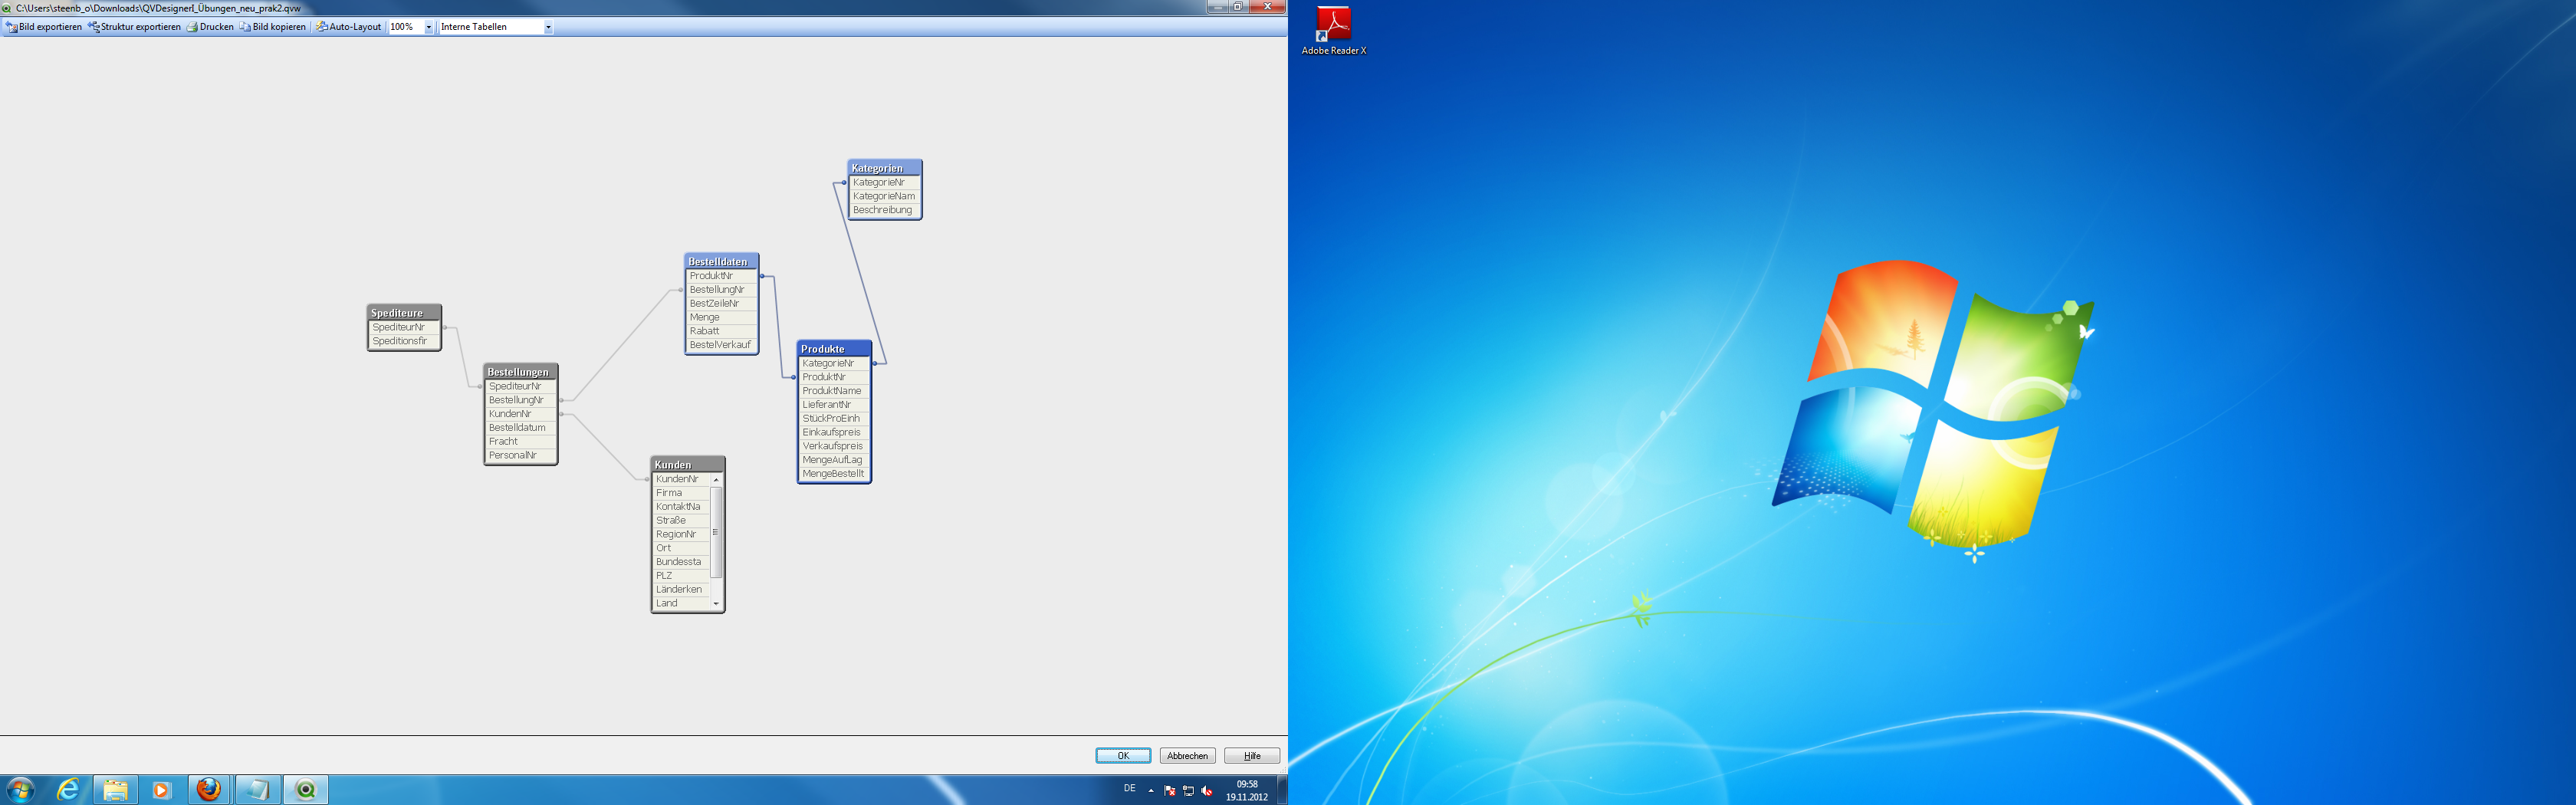
\includegraphics[scale=0.55]{datenmodell1.png}
	\caption{Datenmodell Aufgabe 2} 
\end{turn}
\end{figure}

\end{document}

